\chapter{Vers une génération de rapports automatique à partir d’imagerie avec MyoQuant}
\section{Contexte}
Les outils présentés précédemment ont pour vocation de traiter et d'explorer les comptes-rendus de biopsie textuels. Permettant ainsi une approche rétrospective de l'ensemble des patients connu à ce jour. Cependant il est intéressant d'explorer aussi comment l'analyse d'images par \gls{ia} peut permettre de générer automatiquement ces comptes-rendus de biopsie. Cette approche permettrait un précision et de temps dans l'évaluation des biopsies. Tout d'abord un gain de temps car une approche par \gls{ia} permettrait de traiter  plusieurs biopsie de grand taille de manière automatique, libérant ainsi le temps utilisé pour l'évaluation des coupes histologiques.  Ensuite un gain de précision car, l'évaluation des biopsie par un expert humain est en général qualitative. La description de phénotype se limite généralement à des adjectifs de quantité tel que "peu", "moyen" ou "beaucoup". Grâce à une approche de comptage par \gls{ia}, il est alors possible d'obtenir la quantité précise de fibres présentant un noyau centralisé par exemple et ainsi de pouvoir établir des seuils pour une analyse plus approfondie.

MyoQuant, l'outil présenté dans ce chapitre, est une suite de méthodes pour quantifier différents marqueurs pathologiques dans les biopsies de myopathies congénitales. MyoQuant intègre soit des méthodes algorithmiques simples basée sur des modèles d'\gls{ia} généralistes en histologie comme CellPose (\cite{stringer_cellpose_2021}) et Stardist (\cite{weigert_star-convex_2020}), soit des méthodes basées sur des modèles \gls{ia} développés à partir de nos données. Actuellement, MyoQuant est capable de quantifier des marqueurs pathologiques dans trois des cinq colorations réalisées en routine lors du diagnostic des myopathies congénitales: la centralisation des noyaux à la coloration \gls{he}, un déséquilibre dans le ratio des fibres de type 1 et 2 à la coloration ATPase et une répartition anormales des mitochondries dans les fibres musculaires à la coloration \gls{sdh}. Dans ce chapitre nous allons voir comment ont été implémentées ces solutions de quantifications automatique et des exemples d'application.

\begin{figure}[htbp]
 \centering
 
\includegraphics[width=0.66\textwidth]{figures/myoquant_logo.png}
 \caption[Logo MyoQuant]{Logo de MyoQuant}
 \label{fig:myoquant_logo}
\end{figure}

\section{Analyse de la position des noyaux cellulaires}
Dans un premier temps, nous nous sommes intéressé à l'analyse de la position des noyaux cellulaires dans les fibres musculaire. Dans un muscle sain, les noyaux sont en général en périphérie des fibres, chez les patients atteint de \gls{mc} et particulièrement dans les \gls{cnm}, les noyaux peuvent être internalisés voir centralisés. Par exemple, dans la figure \ref{fig:he_example}, on observe un nombre important de fibre ayant un noyau cellulaire internalisé. Nous avons alors développé une méthode pour compter automatiquement le nombre de fibre présentant un noyau internalisé.
\begin{figure}[htbp]
 \centering
 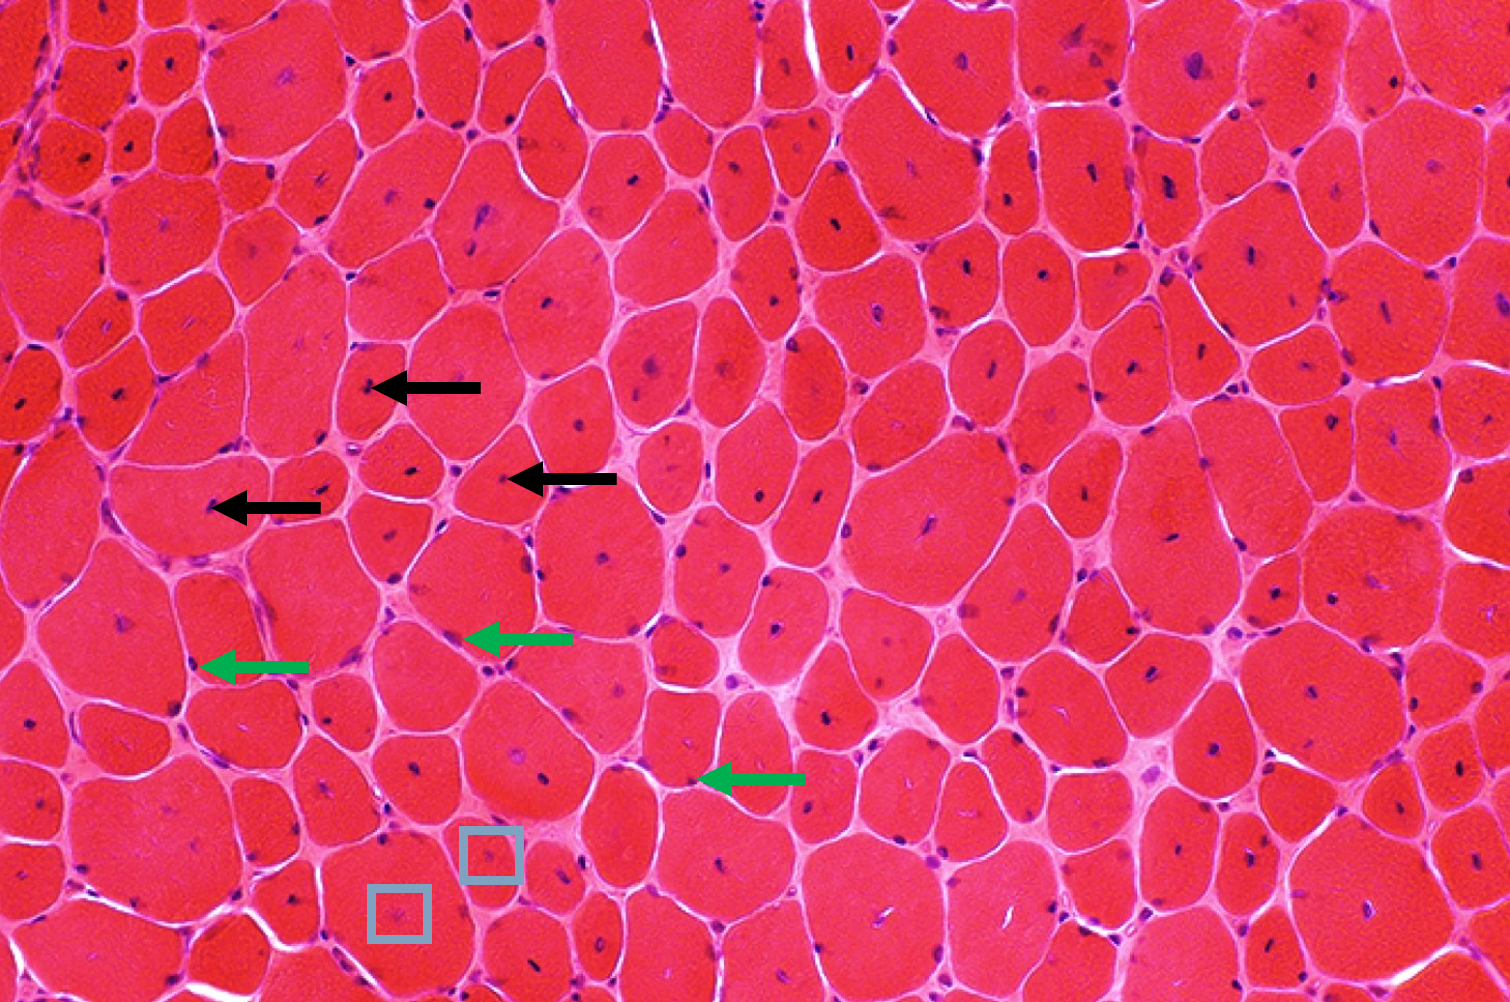
\includegraphics[width=0.8\textwidth]{figures/he_example.jpg}
 \caption[Exemple de biopsie musculaire à la coloration HE]{Exemple de biopsie musculaire de CNM à la coloration HE dans laquelle on observe des fibres avec des noyaux centralisés.}
 \label{fig:he_example}
\end{figure}

\subsection{Algorithme de quantification}
Pour réaliser cette quantification, la première étape consiste à segmenter, c'est à dire obtenir la position de toutes les fibres musculaires et les noyaux de la coupe. Pour cela nous avons utilisés deux modèles d'intelligence artificielle généralistes développés spécifique pour l'analyse de coupe histologique: Cellpose et Stardist. Cellpose nous a permis de segmenter les fibres musculaire, tandis que Stardist nous a permis de segmenter les noyaux cellulaires. La figure \ref{fig:he_seg} présente les résultat de la segmentation de la biopsie présentée en figure \ref{fig:he_example}. On observe que globalement toutes les fibres musculaires sont bien segmentées, cependant concernant les noyaux cellulaires, certains sont trop peu colorés pour être reconnu par le modèle. C'est notamment le cas pour quelques noyaux centraux sur la gauche de la biopsie. Ce qui sera problématique lors de l'analyse des noyaux, car ils ne seront pas considérés.
\begin{figure}[htbp]
 \centering
 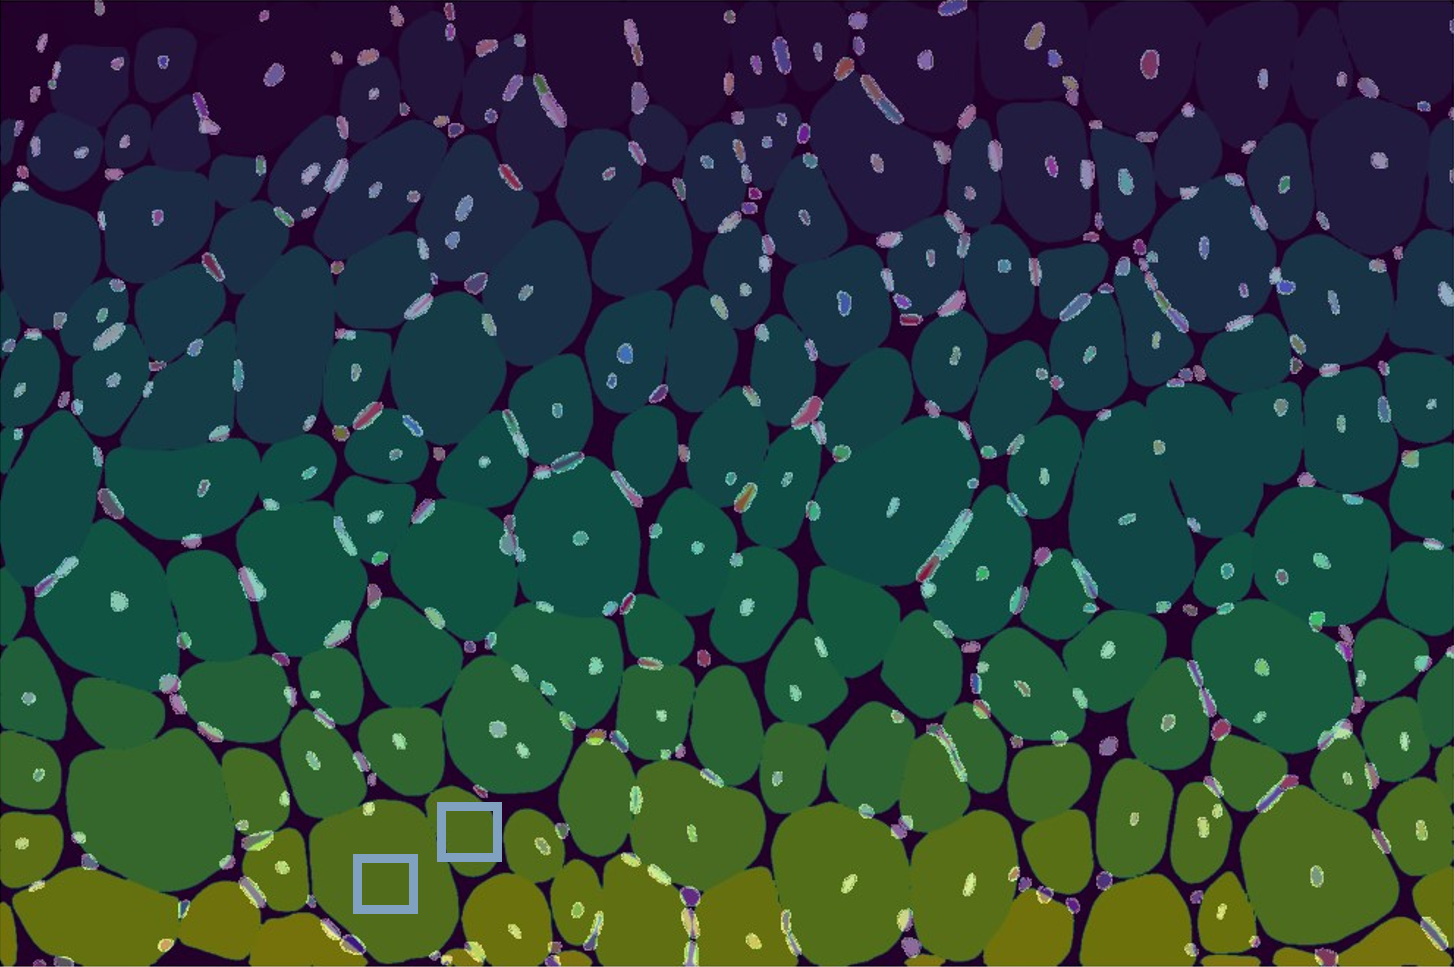
\includegraphics[width=0.8\textwidth]{figures/he_seg.png}
 \caption[Exemple de segmentation de biopsie par Cellpose et Stardist]{Exemple de segmentation des fibres musculaires et des noyaux cellulaires par Cellpose et Stardist}
 \label{fig:he_seg}
\end{figure}

Une fois avoir obtenu la position de chaque fibre et noyaux, nous évaluons la position de chaque noyaux, fibre par fibre. Cette evaluation repose sur le calcul de ce que l'ont appelle un score d'excentricité. Ce score est calculé selon la formule suivante:

\(\text{Score d'excentricité} = \frac{\text{Dist. centre fibre et noyau}}{\text{Dist. centre fibre et membrane}}\)

Où la notation "Dist. centre fibre et noyau" représente la distance en pixels entre le centroïde de la fibre musculaire au centroïde du noyau considéré. Et la notation "Dist. centre fibre et membrane" représente la distance entre le centroïde de la fibre musculaire à la membrane cellulaire selon une droite passant par le noyau d'intérêt. La figure \ref{fig:he_single_nuc}  présente la classification des noyaux d'une fibre musculaire unique. Quatres noyaux ont été détecté dans cette fibre dont trois ont un score d'excentricité supérieur à 0,9 et un inférieur à 0,1. En fixant un seuil de façon empirique à 0,75, on considère alors que cette fibre musculaire possède un noyau internalisé.
\begin{figure}[htbp]
 \centering
 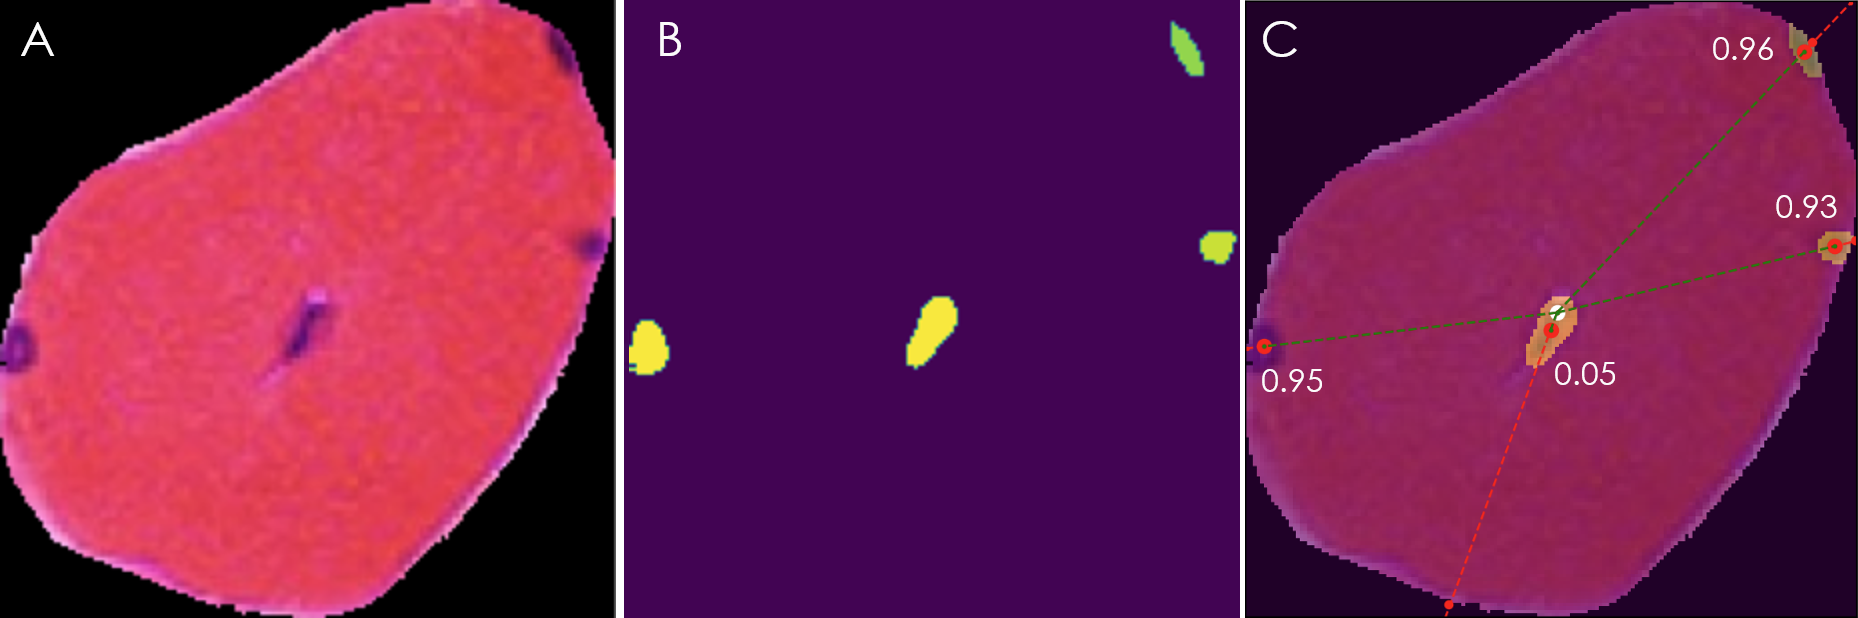
\includegraphics[width=1\textwidth]{figures/he_single_nuc.png}
 \caption[Exemple de classification de la position des noyaux]{Exemple de classification de la position des noyaux cellulaire d'une fibre musculaire. \textbf{(A)} La fibre musculaire seule,\textbf{ (B)} le masque de segmentation des noyaux, 4 pour cette fibre,\textbf{ (C)} schéma de la classification des noyaux avec le score d'excentricité de chaque noyau représentant le ratio de distance: centre de la fibre - noyau vs centre de la fibre - membrane cellulaire.}
 \label{fig:he_single_nuc}
\end{figure}
En comparant l'ensemble des noyaux de chaque fibre à un seuil (ici fixé à 0,75) on peut alors quantifier le nombre de fibre musculaire ayant au moins un ou plusieurs noyaux internalisés. Par exemple pour l'image présenté en figure \ref{fig:he_example}, la figure \ref{fig:he_paint} présente les résultats de classification. Sur cette coupe histologique, on obtient un total de 74 fibres (soit 42\% des fibres) avec au moins un noyau internalisé.
\begin{figure}[htbp]
 \centering
 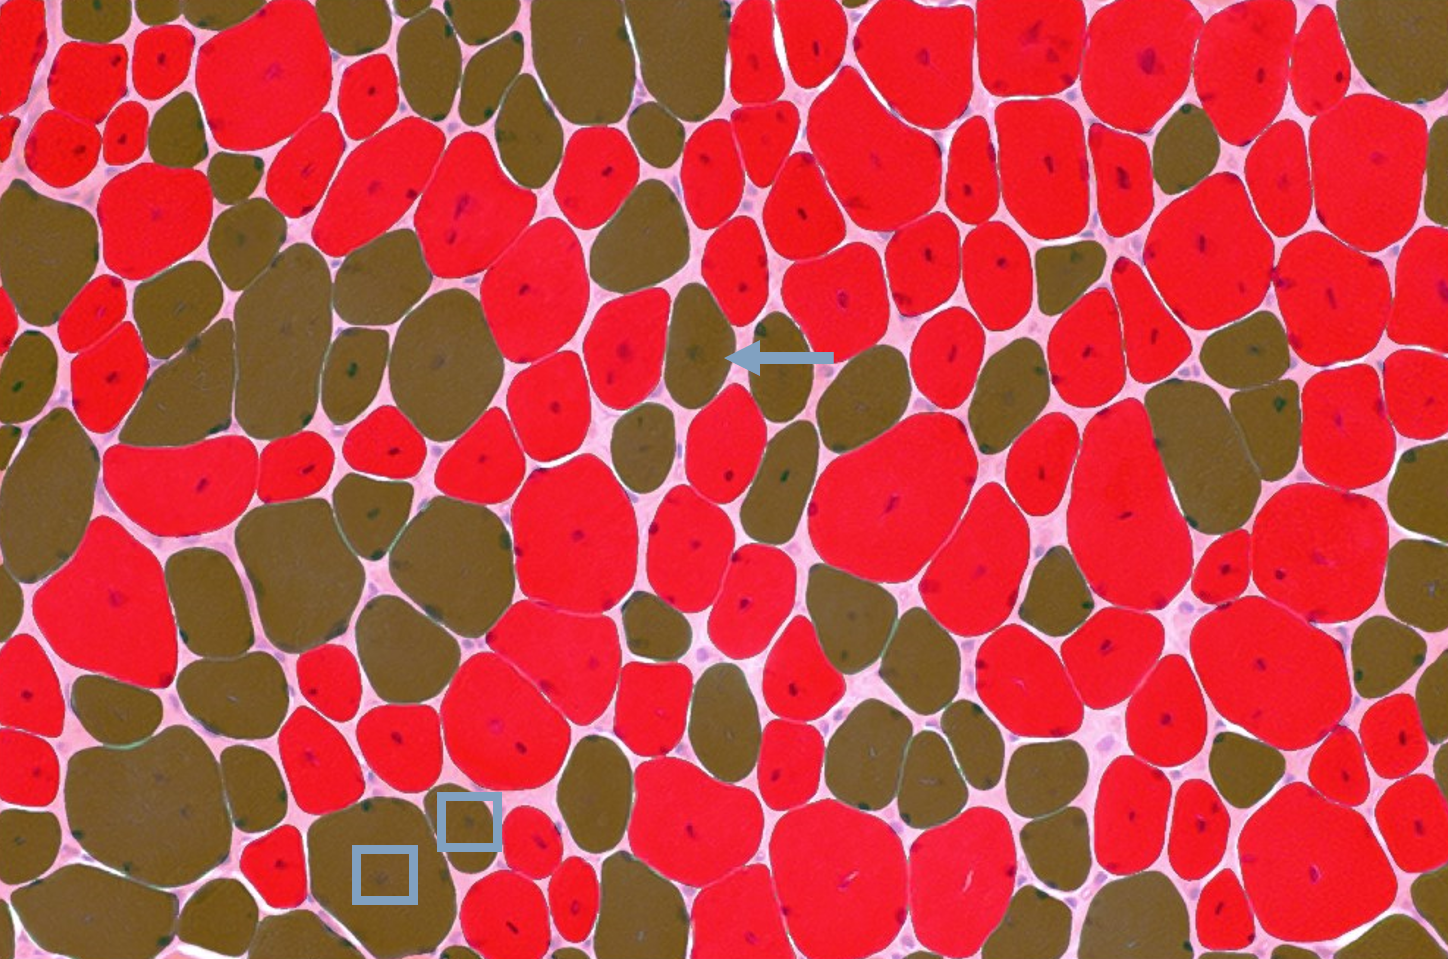
\includegraphics[width=0.8\textwidth]{figures/he_paint.png}
 \caption[Exemple de classification de biopsie musculaire HE]{Exemple de classification de biopsie musculaire à la coloration HE. Colorée en vert les fibres sans noyau internalisé, en rouge les fibres avec au moins un noyau internalisé (score d'excentricité inférieur à 0.75)}
 \label{fig:he_paint}
\end{figure}

\subsection{Exemple d'application: quantification de la régénération musculaire }
La présence de noyaux centralisé dans les fibres musculaire est un marqueur pathologique des les biopsie de myopathies congénitales. Cependant cette centralisation peut aussi être synonyme de régénération musculaire chez les individus sains. Ainsi, la quantification du nombre de noyaux centralisés est donc aussi un moyen de quantifier la régénération musculaire dans une coupe histologique. Ainsi dans le cadre d'une collaboration avec l'\gls{igbmc} et spécifiquement avec l'équipe Biologie moléculaire et cellulaire des cancers du sein du Dr. Tomasetto, nous avons utilisé MyoQuant pour évaluer la quantité de régénération musculaire chez des souris traitée avec un drogue induisant le processus régénération. Ces images d'histologie sont des images à fluorescence (et non à la coloration \gls{he}) avec un fluorochrome pour la membrane cellulaire et un fluorochrome pour les noyaux cellulaire. L'algorithme de MyoQuant est directement compatible avec les images à fluorecence et fonction de la même façon que pour les images à coloration\gls{he}
\begin{figure}[htbp]
 \centering
 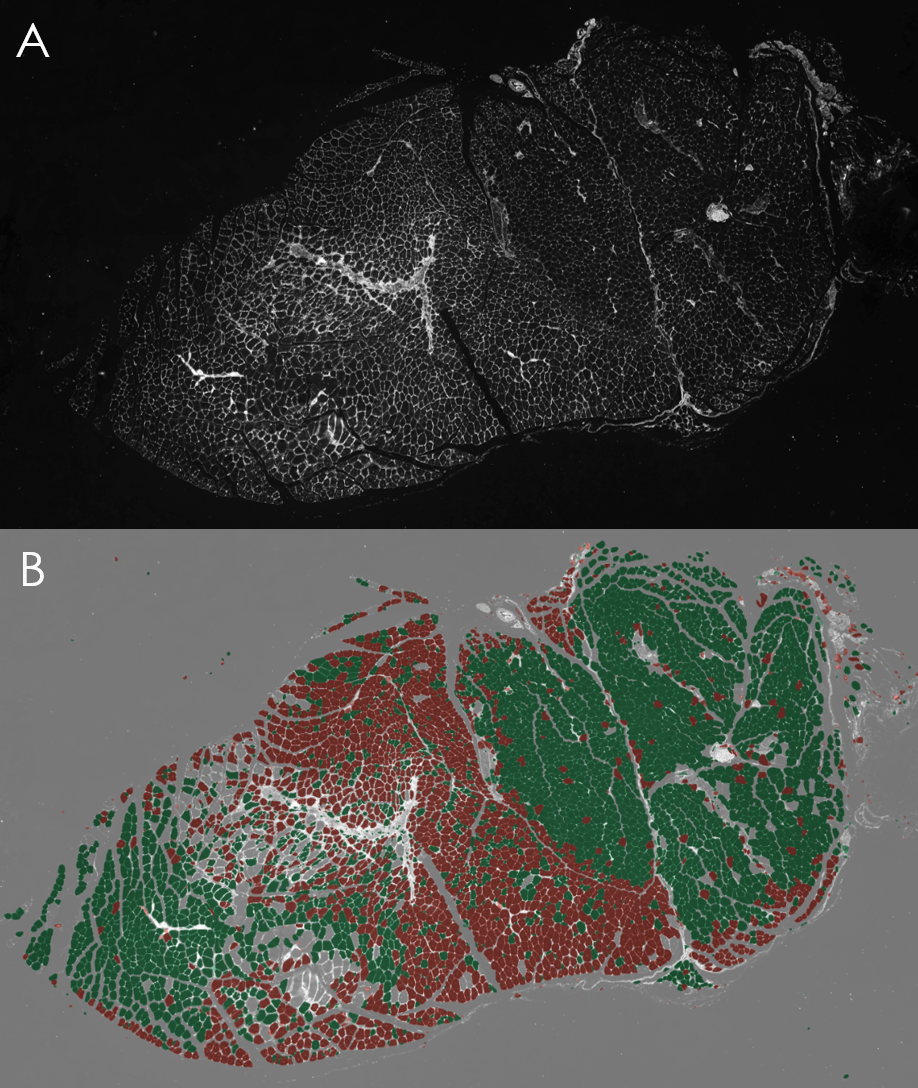
\includegraphics[width=0.8\textwidth]{figures/fluo_nuc.png}
 \caption[Exemple de classification de biopsie musculaire pour la régénération musculaire]{Exemple de classification de biopsie musculaire pour la régénération musculaire. Colorée en vert les fibres sans noyau internalisé (fibre normales), en rouge les fibres avec au moins un noyau internalisé (en régénération)}
 \label{fig:fluo_paint}
\end{figure}

La figure \ref{fig:fluo_paint} présente un exemple de coupe complète de biopsie musculaire de souris avec le masque de quantification associé généré par MyoQuant. Sur cette image, il y a 6078 fibres musculaires détectées, dont 2285 (environ 35\%) sont en régénération. Le tableau \ref{tab:myoquant_fluo_time} présente le temps de calcul nécessaire pour chaque étape de la quantification pour la coupe \ref{fig:fluo_paint} et le tableau \ref{tab:myoquant_fluo_results} présente les résultats de cet quantification. On observe ici que pour traiter  une coupe complète sur une machine sans matériel spécifique (sans GPU) il a nécessité environ 1 heure de calcul, dont la majorité a été utilisée par Cellpose pour segmenter les fibres musculaire. Cependant cette vitesse peut-être largement améliorée d'un facteur 5 par l'utilisation de matériel spécifique aux calculs \gls{ia} (GPU), passant de 3782 secondes pour Cellpose à 652. Pour une image contenant 6078 fibres et 23 628 noyaux, cela représente environ 1.6 fibre traitée par seconde. Cette quantification a mis en évidence que 37\% des fibres présentaient un noyau internalisé et donc sont en régénération.
\begin{table}[ht]
\centering
\caption{Temps de calcul pour l'analyse des noyaux d'une coupe complète (6078 fibres, 12000 x 9600 pixels)}
\label{tab:myoquant_fluo_time}
\begin{tabularx}{\textwidth}{|X|X|X|X|}
\hline
\textbf{Etape} & \textbf{Temps sur GPU} & \textbf{Temps sur CPU (s)} & \textbf{Fibre par seconde (sur CPU)} \\
\toprule
Cellpose & 652 & 3 782 & 1.6 \\
\hline
StarDist & \textit{out-of-memory} & 21 & 29 \\
\hline
Classification des noyaux & 68 & 68 & 89 \\
\hline
\textbf{Total} & \textbf{>720} & \textbf{3 871} & \textbf{1.57} \\
\hline
\end{tabularx}
\end{table}
\begin{table}[ht]
\centering
\caption{Résultats de quantification des noyaux d'une coupe complète (6078 fibres, 12000 x 9600 pixels)}
\label{tab:myoquant_fluo_results}
\begin{tabularx}{\textwidth}{|X|X|X|}
\hline
\textbf{Type} & \textbf{Valeur} & \textbf{Proportion (\%)} \\
\toprule
N° Fibre & 6 078 & 100 \\
\hline
N° Fibre avec 1+ noyau internalisé & 2 264 & 37 \\
\hline
\hline
N° Noyaux & 23 628 & 100 \\
\hline
N° Noyaux internalisés & 3 933 & 16 \\
\hline
N° Noyaux périphériques & 17 918 & 76 \\
\hline
N° Noyaux non-classés (hors fibres) & 1 777 & 8 \\
\hline
\end{tabularx}
\end{table}
Le tableau \ref{fig:fluo_compil} présente l'ensemble des quantification opérée dans les différentes conditions de traitement et de génotype (au total 35 \gls{wsi} analysées). On observe qu'après traitement avec la \textit{Cardiotoxin}, une drogue induisant la régénération musculaire, une proportion significativement supérieur de fibre ayant un noyaux internalisé par rapport aux coupes contrôle. Ces résultats confirment que MyoQuant est bien capable d'évaluer de façon robuste la présence de noyaux internalisés, un marqueur de la régénération musculaire.

\begin{figure}[htbp]
 \centering
 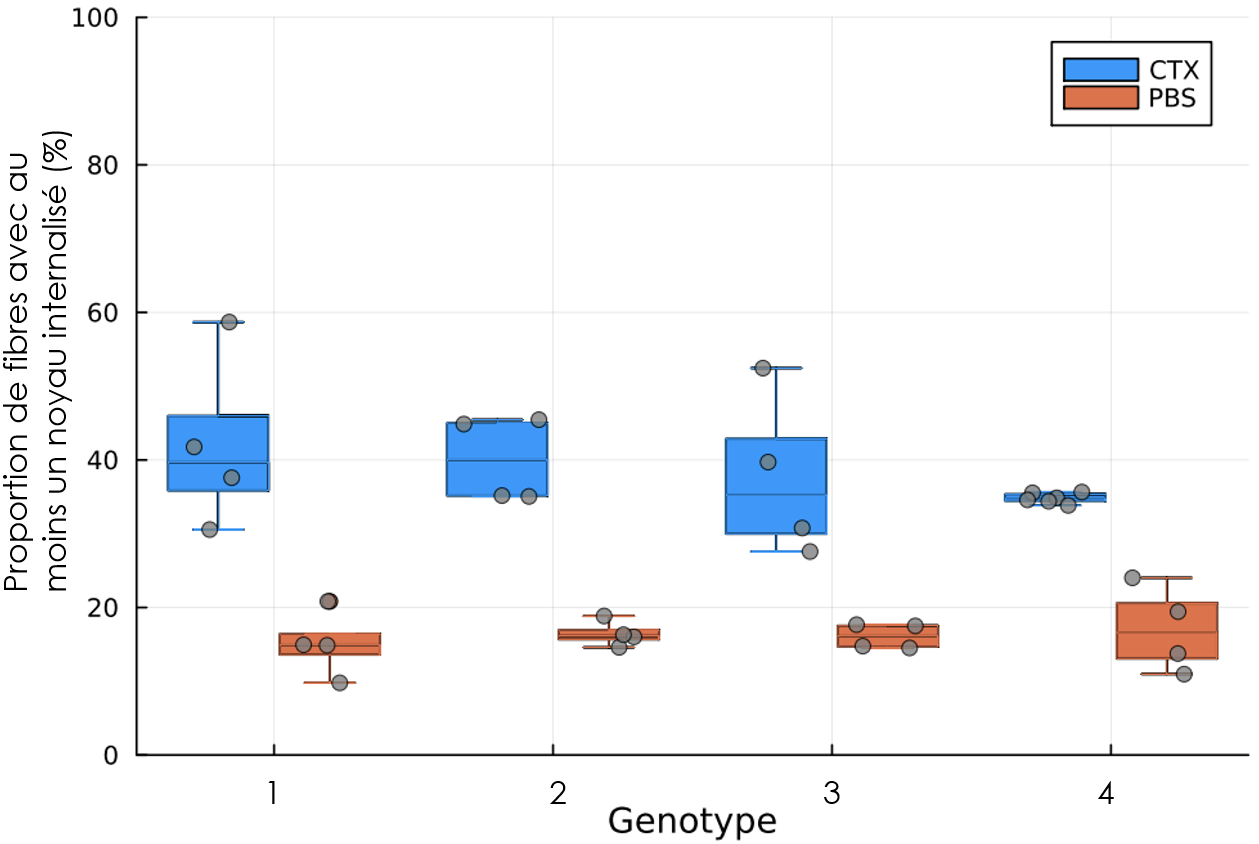
\includegraphics[width=0.8\textwidth]{figures/fluo_compil.png}
 \caption[Résultat de la quantification de la régénération musculaire]{Résultat de la quantification de la régénération musculaire chez des souris pour 4 génotype différents traité (bleu) ou non (orange) avec une drogue induisant la régénération musculaire.}
 \label{fig:fluo_compil}
\end{figure}

\section{Ratio de fibre de type 1 et 2: classification basée sur l'intensité de coloration}

Dans un second temps, nous nous sommes intéressé à l'analyse du ratio des différents type de fibre musculaire dans les biopsies. Dans certaines myopathies congénitales, l'équilibre entre fibre de type 1 et type 2 peut-être modifié avec une prédominance des fibres de type 1. Les différents type de fibre musculaire sont colorée différentiellement (différence d'intensité) à la coloration ATPase. A un pH 4.3, les fibres de type 1 sont sombres et les fibres de type 2 sont pales, et inversement au pH 9.4. La figure \ref{fig:atp_example} représente une biopsie musculaire colorée à l'ATPase pH 9.4. On observe la présence de deux populations de fibres à coloration distinctes. Nous avons alors développé une méthode pour compter automatiquement le nombre de fibre de chaque type.
\begin{figure}[htbp]
 \centering
 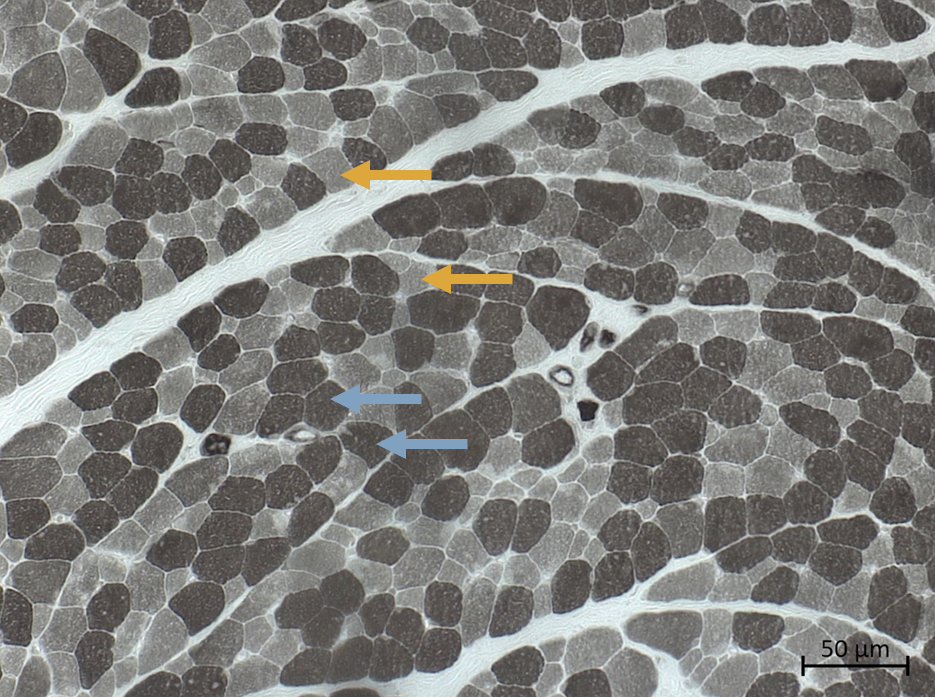
\includegraphics[width=0.8\textwidth]{figures/atp_example.png}
 \caption[Exemple de biopsie musculaire à la coloration ATPase pH 9.4]{Exemple de biopsie musculaire à la coloration ATPase pH 9.4 qui permet de différencier les fibres de type 1 aux fibres de type 2.}
 \label{fig:atp_example}
\end{figure}
\subsection{Algorithme de quantification}
Pour réaliser cette quantification, la première étape consiste à segmenter, c'est à dire obtenir la position de toutes les fibres musculaires. Comme précédemment, nous avons utilisés Cellpose afin segmenter les fibres musculaire. Ensuite pour chaque fibre nous avons extrait l'intensité moyenne de la fibre et avons réalisé un histogramme. La figure \ref{fig:atp_density} présente l'histogramme issue de l'analyse de l'image d'exemple pour la coloration ATPase pH 9.4 (\ref{fig:atp_example}). Le but de la procédure est de déterminer automatiquement les pics présent dans l'histogramme et de trouver les minimums locaux entre les pics pour fixer un ou plusieurs seuil d'intensité. Pour cela, à partir des valeurs de cet histogramme, une courbe de densité est créée (par méthode de \gls{kde}). Puis à partir de cette courbe de densité, une méthode de mélange Gaussien est utilisée pour déterminer la position des pics dans la courbe de densité. Finalement, le seuil est déterminé en trouvant le minimum local de la courbe de densité entre les deux pics.
\begin{figure}[htbp]
 \centering
 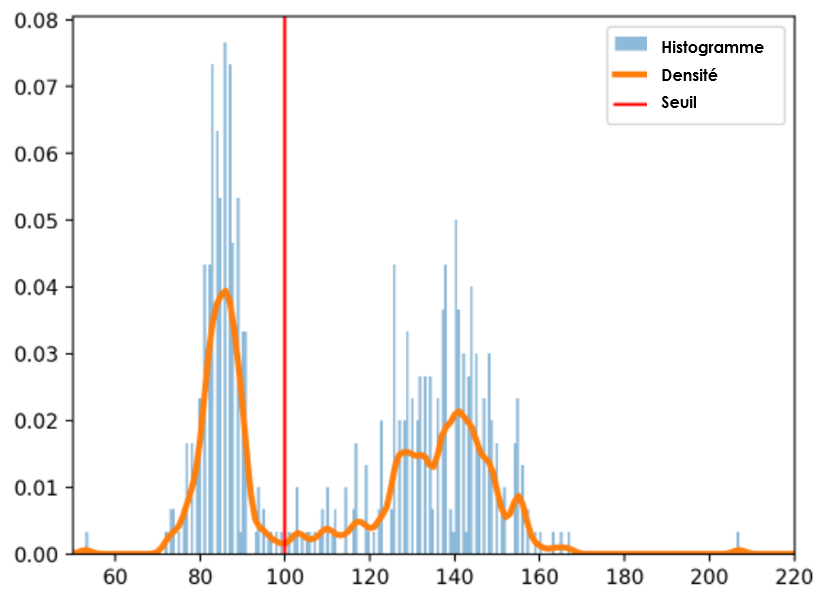
\includegraphics[width=0.8\textwidth]{figures/density_plot.png}
 \caption[Exemple d'histogramme et courbe de densité biopsie ATPase]{Exemple d'histogramme et courbe de densité biopsie ATPase}
 \label{fig:atp_density}
\end{figure}

A partir de ce seuil, il est alors possible de classer les fibres musculaire en deux catégories: celle avec une intensité moyenne inférieure au seuil et celle avec une intensité moyenne supérieure. La figure \ref{fig:apt_paint} présente les résultat de la quantification automatique des fibres de l'image présenté en exemple précédemment. Sur cette images, on a pu quantifier au total la présence de 496 fibres, dont 269 (54\%) fibres de type 1 et 227 (46\%) fibres de type 2. 
\begin{figure}[htbp]
 \centering
 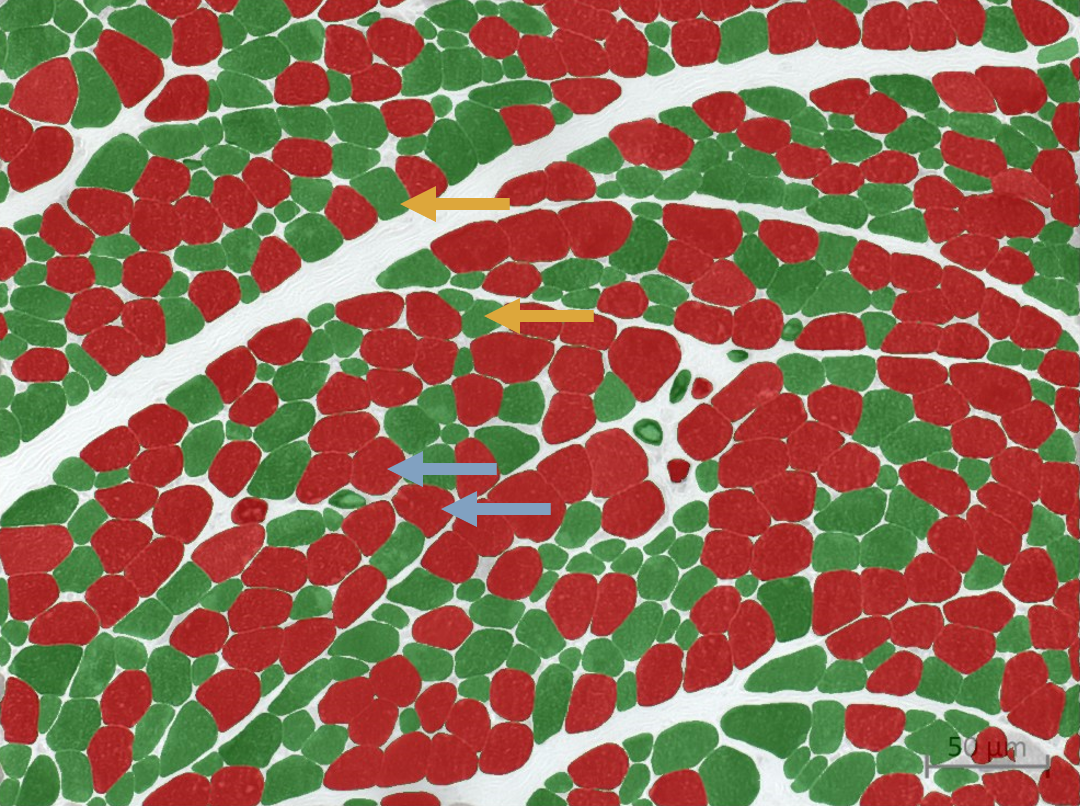
\includegraphics[width=0.8\textwidth]{figures/atp_paint.png}
 \caption[Exemple de classification de biopsie musculaire à la coloration ATPase]{Exemple de classification de biopsie musculaire à la coloration ATPase. Colorée en rouge les fibres ayant une intensité inférieur au seuil (type 2) en vert supérieur au seuil (type 1)}
 \label{fig:apt_paint}
\end{figure}

\subsection{Exemple d'application: classification d'une coupe complète avec trois types de fibre}
La coloration ATPase peut révéler plus de deux types de fibre musculaire. En effet les fibre type 2 ont plusieurs sous-type visualisation dans certaines conditions de colorations. Dans cet exemple, nous avons utilisé la méthode de classification développé pour détecter trois types de fibres. L'algorithme présenté dans cette section est capable d'établir autant de seuil automatiquement que spécifié par l'utilisateur (et non pas seulement deux). La figure \ref{fig:atp_paint_wsi} présente les résultats de classification d'une \gls{wsi} de biopsie musculaire colorée à l'ATP pH 9.4. Sur cette coupe on observe trois populations de fibres: des fibres pâles (fibre de type 1), des fibres sombres (fibre de type 2A) et de petites fibres très sombres localisée en haut de la coupe (fibre type 2B). La méthode de quantification a alors pu définir deux seuils pour séparer ces trois classes. 
\begin{figure}[htbp]
 \centering
 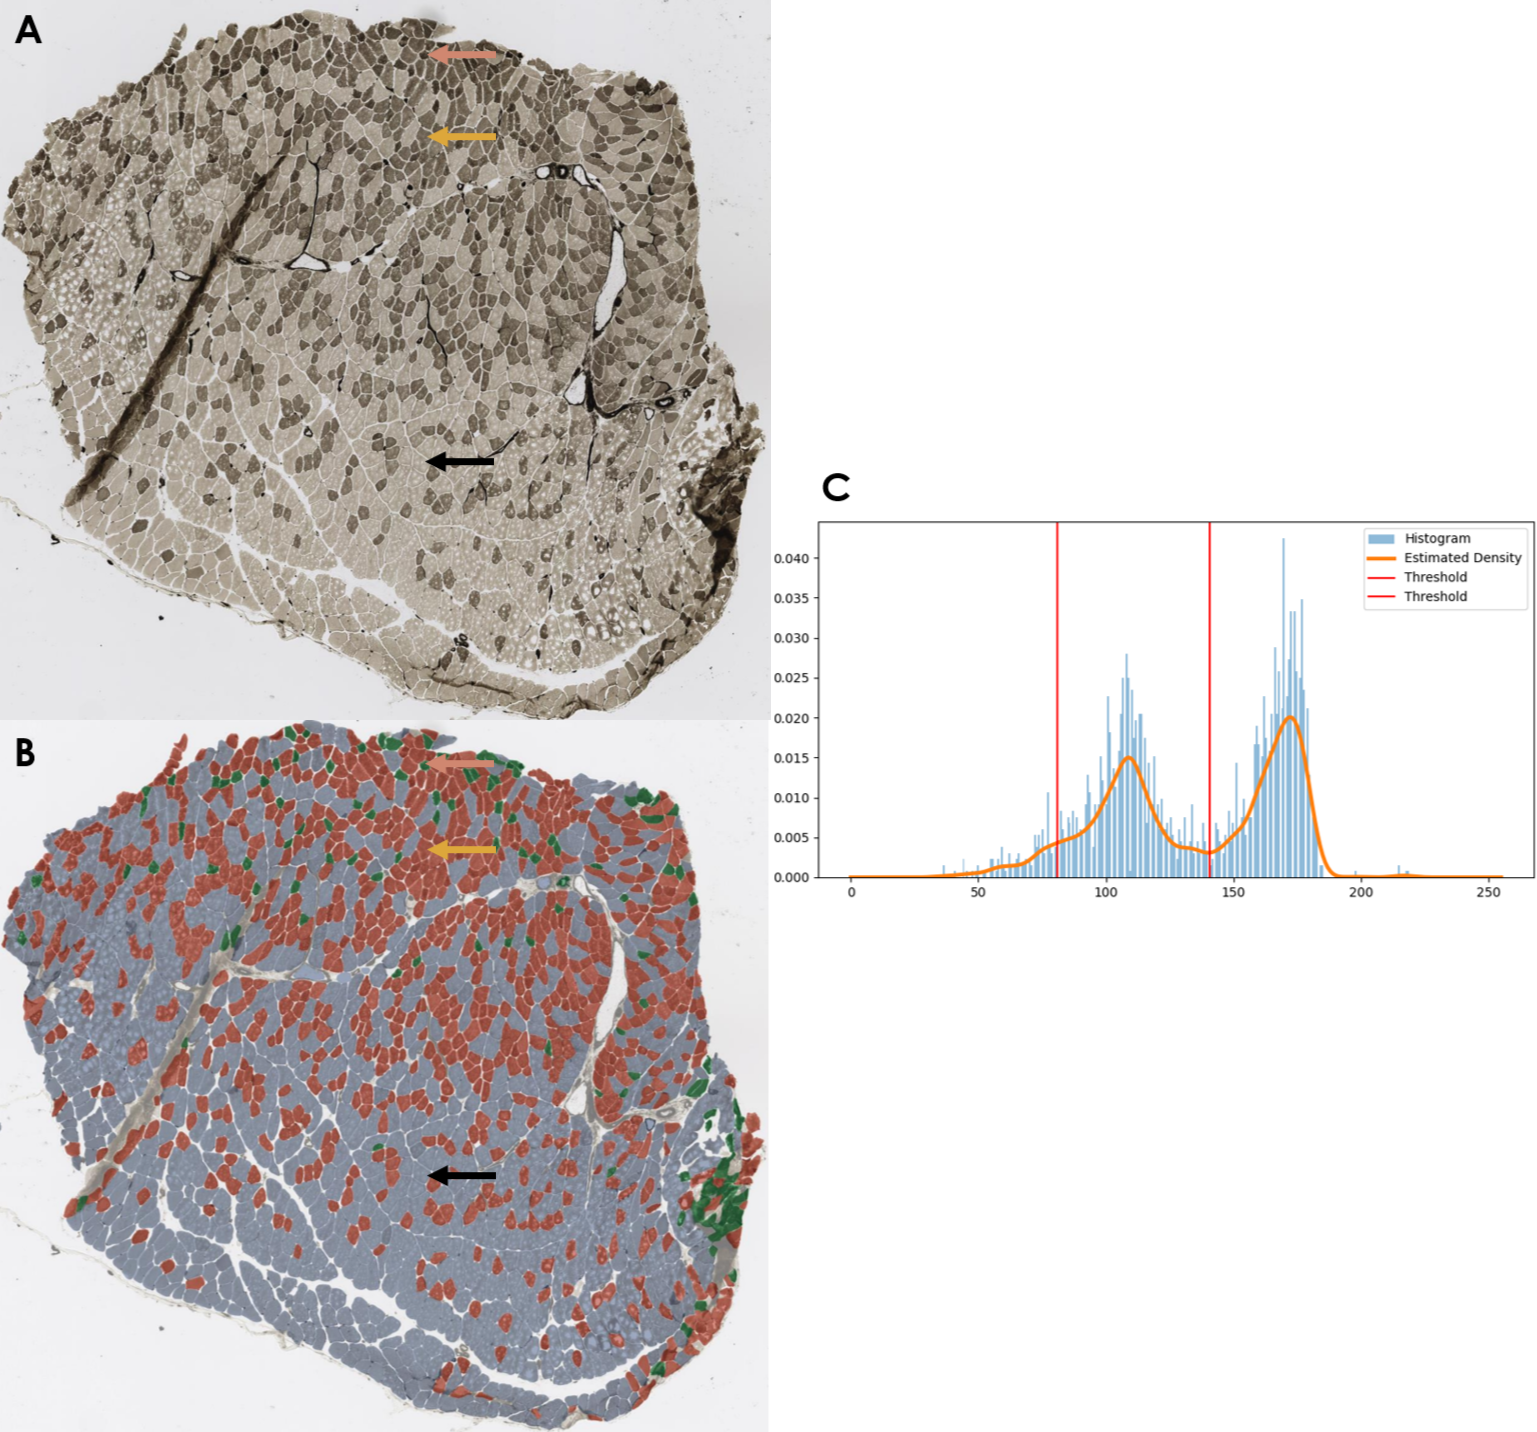
\includegraphics[width=1\textwidth]{figures/atp_wsi.png}
 \caption[Exemple de classification de biopsie musculaire pour la régénération musculaire]{Exemple de classification de biopsie musculaire pour la régénération musculaire. Colorée en vert les fibres sans noyau internalisé (fibre normales), en rouge les fibres avec au moins un noyau internalisé (en régénération)}
 \label{fig:atp_paint_wsi}
\end{figure}

Les résultats de cette classification sont référencé dans le tableau \ref{tab:atp_wsi_resultstable} , le temps de calcul et la vitesse de classification sont disponibles dans le tableau \ref{tab:atp_wsi_timetable}. Au total, 1840 fibres ont été classifiée en 131 secondes (soit 14 fibres par secondes). Il y a une majortié de fibre de type 1 (894, 49\%), de fibre de type de 2A (829, 45\%) et une faible proportion de petite fibre de type 2B (117, 6\%). Les résultats de cette quantification sont visuellement satisfaisant, bien qu'une partie de la biopsie en bas a droite, est repliée sur elle même et donc apparaît avec une intensité de coloration forte. Cette zone a donc été considérée à tort comme des fibres de type 2B. Ces résultats mettent en évidence le besoin biopsie avec une préparation de qualité pour obtenir des résultats robustes lors de la quantification automatique.

\begin{table}[ht]
\centering
\caption{Temps de calcul pour l'analyse des types de fibre d'une coupe complète (1840 fibres, 6000 x 5600 pixels)}
\label{tab:atp_wsi_timetable}
\begin{tabularx}{\textwidth}{|X|X|X|}
\hline
\textbf{Étape} & \textbf{Temps sur GPU} & \textbf{Fibre par seconde (sur GPU)} \\
\toprule
Cellpose & 113 & 16 \\
\hline
Classification des fibres & 18 & 102 \\
\hline
\textbf{Total} & \textbf{131} & \textbf{14} \\
\hline
\end{tabularx}
\end{table}
\begin{table}[ht]
\centering
\caption{Résultats de quantification des types de fibre d'une coupe complète (1840 fibres, 6000 x 5600 pixels)}
\label{tab:atp_wsi_resultstable}
\begin{tabularx}{\textwidth}{|X|X|X|}
\hline
\textbf{Type} & \textbf{Valeur} & \textbf{Proportion (\%)} \\
\toprule
Fibre type 1 & 894 & 49 \\
\hline
Fibre type 2A & 2 829 & 45 \\
\hline
Fibre type 2B & 117 & 6 \\
\hline
\end{tabularx}
\end{table}


\section{Répartition des mitochondrie: classification basée sur intelligence artificielle}
* présentation du problême
\subsection{Jeu de donnée de souris et annotations}
\subsection{Entrainnement et architecture de l'IA}
\subsection{ Performance et explicabilité de l'IA}
\subsection{Exemple d'application}
\subsection{Exploration du modele}
* Embedding des images / PCA / features extraites par modèles par trucs
* Performance supérieure à l'Homme ; Correction des annotations / identitifaction


\section{Déploiement de la plateforme}
\subsection{Outil en ligne de commande}
* Traitement de grande quantitté d'images et slides complètes mais besoin de GPU la majorité du temps
\subsection{Démo en ligne}
* Pour faire la promotion de l'outil et faire des test sur des morceaux d'images + paramètre visuel + explicabilité
\section{Limitations}
* Entrainé sur la souris, pas toutes les colorations, pas tout les marqueurs pour chaque coloration

\section{Perspectives futures de développement}
* Ajouts de nouvelles colorations et nouveaux marqueurs
* Déploiement d'interface avec accès GPU
* Test grand échelle chez l'Homme pour dataset comparaison expert / humain
* Analyse de vrai patients pour voir si on peut faire des seuil en fonction des diag
* he analyse plus de valeurs à analyse taille + co disponibles